\section{实验发现一：静态评测会改变排序并掩盖记忆退化}

本章结论是：在长程对话记忆评测中，\textbf{off-policy evaluation 会改变 memory agent 的相对排序，并引入 reuse bias}；同时，随着对话推进到后期 period，模型的真实记忆能力会明显下降。若只看表层回答质量，评测者容易低估底层记忆机制已经失效的程度。

\begin{importantbox}{评测模式会改变排序}
对 memory agent 来说，评测方式本身会成为实验变量。沿用前文定义，off-policy evaluation 读取固定轨迹后答题，on-policy evaluation 让 agent 亲自参与轨迹生成。直观类比是：读行车记录后回答路况，与真正开完这段路后再复盘判断，测到的能力范围不同。
\end{importantbox}

\subsection{off-policy 排序会误导记忆系统选择}

视频首先追问的问题是：off-policy evaluation 是否会误导排序。实验图给出的关键现象很直接：AWE 在 on-policy setting 下排第一，到了 off-policy setting 下却降到第三。这说明同一个 memory agent 在不同评测模式中会得到不同的相对位置，配置选择也会随之改变。图~\ref{fig:offpolicy-mislead} 是本节的关键证据，读图时应重点看排序变化，避免过度解读截图里难以辨认的小数值。

\begin{figure}[H]
  \centering
  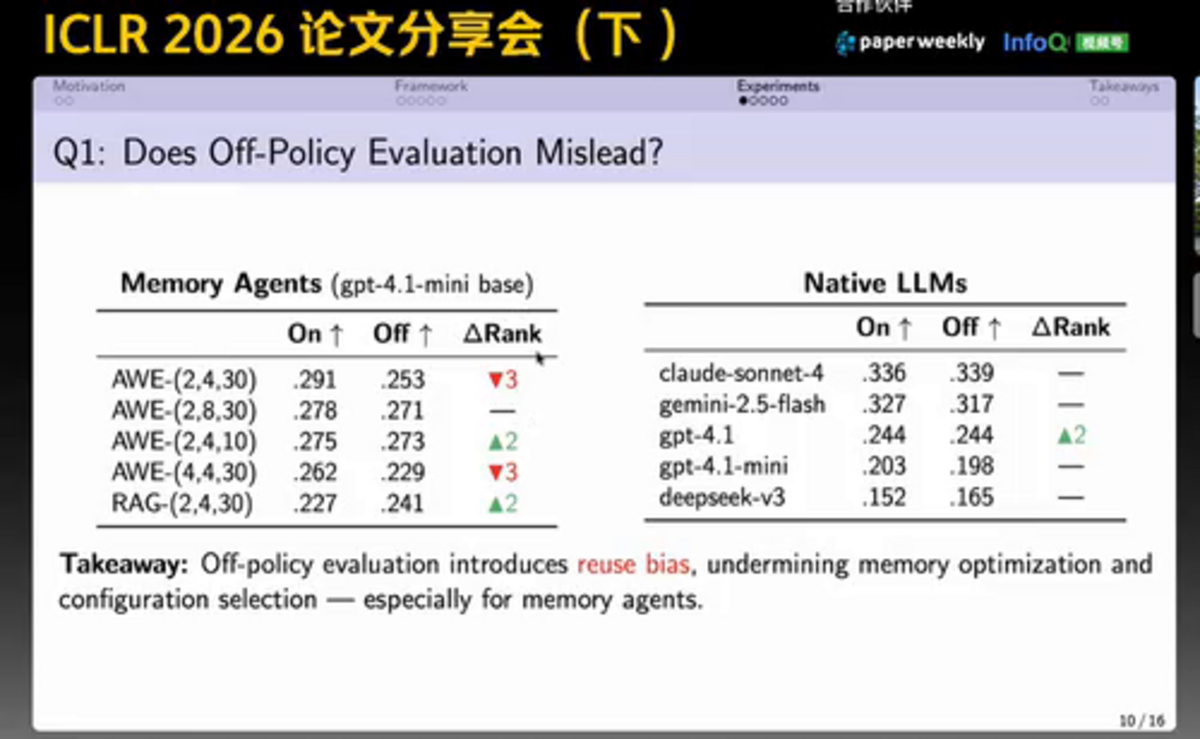
\includegraphics[width=0.82\linewidth,height=0.34\textheight,keepaspectratio]{figures/fig06_offpolicy_mislead.png}
  \caption[off-policy evaluation 改变 memory agent 排序]{off-policy evaluation 会改变 memory agent 的排序，AWE 在 on-policy 下领先，在 off-policy 下下降到第三。\protect\footnotemark}
  \label{fig:offpolicy-mislead}
\end{figure}
\footnotetext{视频时间：00:11:10--00:12:50。}

同一张图还给出 native long-context LLM 的对照：右侧表格的排序变化相对稳定，说明 off-policy 的伤害在这个实验里主要集中于需要评估记忆策略本身的 agent 方案。原因很直接：native model 没有独立 memory-write policy，固定轨迹对它的策略闭环破坏较小；AWE、RAG、AWI 的差异则来自写入、读取和使用链路，静态复用轨迹会直接改变这些链路的发挥空间。

这里的核心问题叫 \textbf{reuse bias}。在 off-policy setting 中，agent 面对的是固定、预先生成的对话，它无法让自身记忆内容反过来塑造下一轮互动。对于 AWE 这类让 agent 自主决定写入外部记忆的机制，这个限制尤其关键，因为它的优势正来自闭环过程中的主动筛选、写入和后续使用。用静态轨迹评价这类系统，相当于把系统最需要发挥作用的反馈路径拿掉，再要求它证明自己的价值。

\begin{warningbox}{配置选择风险}
工程含义很尖锐：如果团队用 off-policy 分数来决定 memory system 配置，可能会错过 on-policy 交互中更有效的方案。排序从第一变成第三已经足够说明，这类评测可直接影响产品选型。
\end{warningbox}

\subsection{后期 period 暴露真实记忆退化}

第二个实验问题转向当前 LLM 在长对话中到底能记住多少。视频展示了两组 heatmap：overall score 和 normalized memory score。这里需要谨慎解读：图中细粒度数值不宜逐格复述，可靠结论是随着 period index 往后推进，记忆表现明显下降。图~\ref{fig:memory-score-heatmaps} 的用途是支持趋势判断，避免逐格抄录实验数字。

\begin{figure}[H]
  \centering
  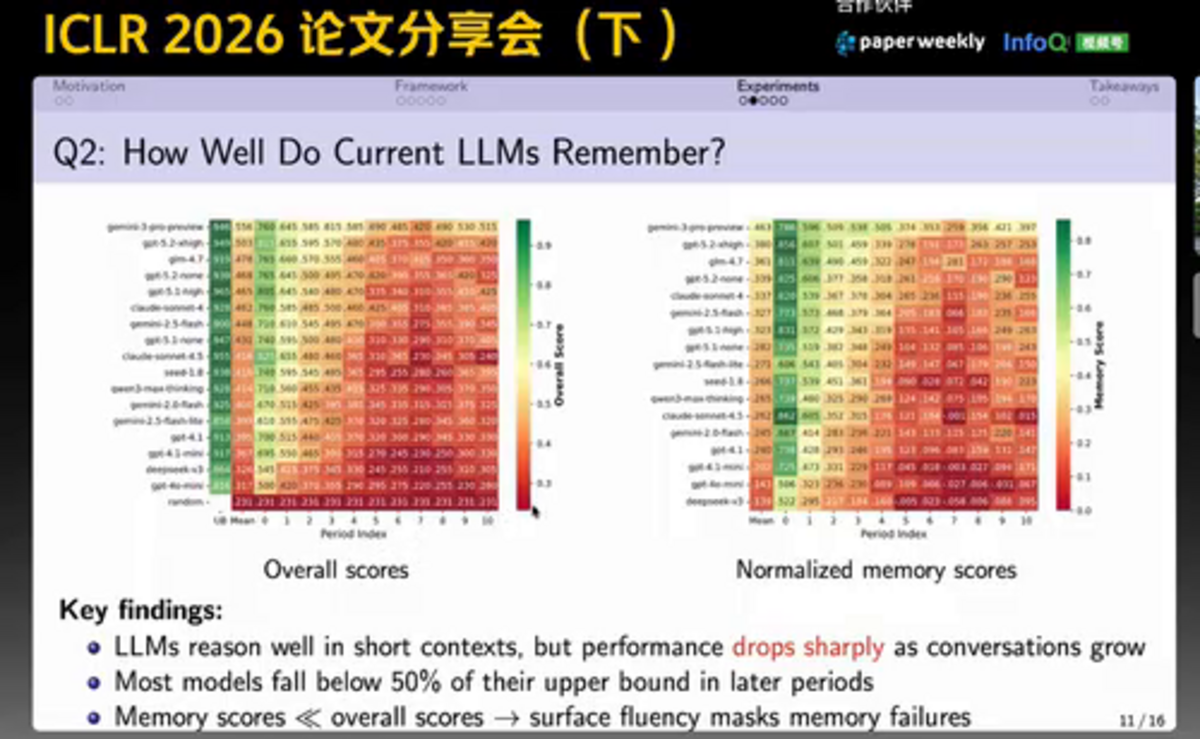
\includegraphics[width=0.82\linewidth,height=0.34\textheight,keepaspectratio]{figures/fig07_memory_score_heatmaps.png}
  \caption[overall score 与 normalized memory score 的 heatmap]{overall score 与 normalized memory score 的 heatmap 显示，后期 period 的记忆能力明显下降。\protect\footnotemark}
  \label{fig:memory-score-heatmaps}
\end{figure}
\footnotetext{视频时间：00:12:50--00:14:15。}

normalized memory score 延续上一章提到的归一化思路：它把表现放在 random baseline 与 perfect memory upper bound 之间观察，可以理解为一把专门量记忆的尺子。它关注模型是否保留了对话中的关键事实、偏好和状态变化。overall score 更像综合印象分，可能受到语言流畅度、推理姿态和回答完整性的影响。视频给出的解释是，模型听起来可以很自信，底层却已经遗忘关键内容。长程对话评测因此要把“会说得顺”和“真的记得住”分开看。

更尖锐的结果是，后期 period 中多数模型的 normalized memory score 会低于 perfect-memory upper bound 的 50\%，有些格子甚至落到 random score 以下。这个说法应作为趋势级结论使用：截图里的单元格数值可读性有限，适合支持“后期记忆塌缩”这一判断，逐格复述精确小数会制造虚假精度。

\subsection{本章小结}

本章的实验发现可以收束为两点。第一，off-policy evaluation 会引入 reuse bias，AWE 在 on-policy 中排第一，在 off-policy 中降到第三，native long-context LLM 排序相对稳定，说明静态评测对 memory agent 的优化方向影响更大。第二，heatmap 显示后期 period 的记忆能力明显下降，许多模型低于 perfect-memory upper bound 的 50\%，有时甚至低于 random score，提示长程对话中的核心风险来自持续记忆退化。ASR 中的 “of policy” 在本章统一校正为 `off-policy`，热力图相关的 “matrix” 按语境写作 `metrics` 或 `heatmap`。

\section{实验发现二：外部记忆的收益取决于写、读、用三环节权衡}

本章结论是：\textbf{external memory 确实能改善长程对话记忆，但收益取决于 write、read、utilization 三个环节之间的权衡}。RAG 和 AWE 能把 utilization failure 从约 24\% 降到约 7\%，同时会带来 write 和 read 错误的上升；AWI 的主要问题是把信息压缩进 context buffer 时会丢失细节。

\begin{knowledgebox}{外部记忆的三种路径}
external memory 可以类比为模型外部的工作笔记。RAG 把完整对话历史放进 vector store，再检索相关片段作为上下文；AWE 让 agent 自主决定哪些信息写入 external memory bank；AWI 把记忆内容压缩进模型自己的 in-context buffer。三者都在帮模型“记东西”，差异在于谁来筛选、记在哪里、之后怎样取出来。
\end{knowledgebox}

\subsection{三类 external memory 的直接对比}

视频将三类实现并排比较：RAG、AWE 和 AWI。RAG 的优点是直接，把完整历史存入外部向量库，回答时再检索相关内容作为 context；风险是检索结果可能 noisy。AWE 的关键动作是 agent 自主决定什么信息值得写入外部 memory bank。AWI 的路径更内向，它把信息压缩到大模型自身的 context buffer 中。图~\ref{fig:external-memory} 把三类路径放在同一页，适合用来对照“谁筛选、存在哪里、怎样读回”。

\begin{figure}[H]
  \centering
  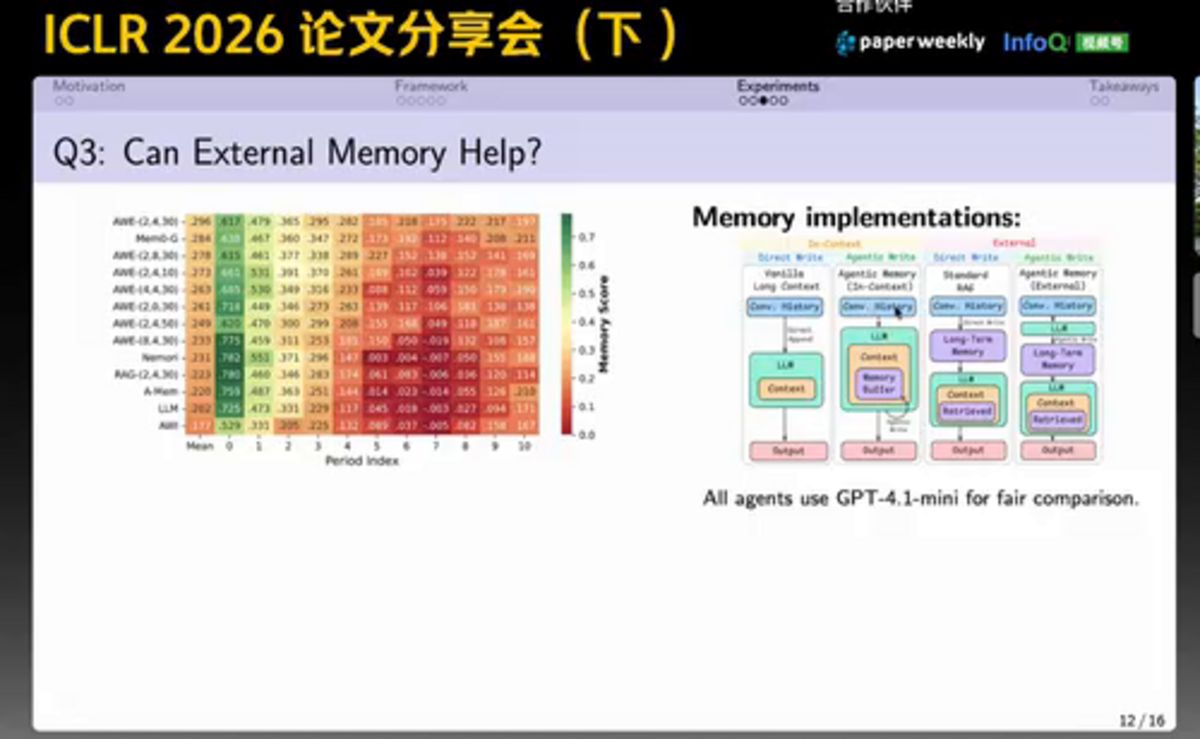
\includegraphics[width=0.82\linewidth,height=0.34\textheight,keepaspectratio]{figures/fig08_external_memory.png}
  \caption[RAG、AWE、AWI 三类 external memory 机制对比]{RAG、AWE、AWI 三类 external memory 机制的对比，视频指出 AWE 在该组比较中表现最好。\protect\footnotemark}
  \label{fig:external-memory}
\end{figure}
\footnotetext{视频时间：00:14:15--00:16:30。}

这组对比中，AWE 的表现最好。直观原因是它让 agent 先做信息筛选，再写入外部记忆；RAG 存得更全，检索时也更容易带入噪声；AWI 在压缩进 buffer 的过程中会损失细节，视频特别指出这种压缩可能让表现变差。该实验强调外部记忆的组织方式：谁来筛选、存在哪里、怎样读回，都会决定后续能否读到、用上关键事实。

\subsection{write、read、utilization 的失败转移}

更细的诊断把失败分为三个环节。write failure 指信息从一开始就没有被记录；read failure 指信息曾被记录，后续检索或读取失败；utilization failure 指系统知道事实，却没有把事实正确用于回答。三者像一条流水线，前面漏掉的内容，后面很难补回来；前面记录了内容，后面也可能取错或用错。图~\ref{fig:failure-tradeoff} 展示的是失败类型之间的转移关系，核心读法是看 utilization failure 下降时 write/read 错误怎样上升。

\begin{figure}[H]
  \centering
  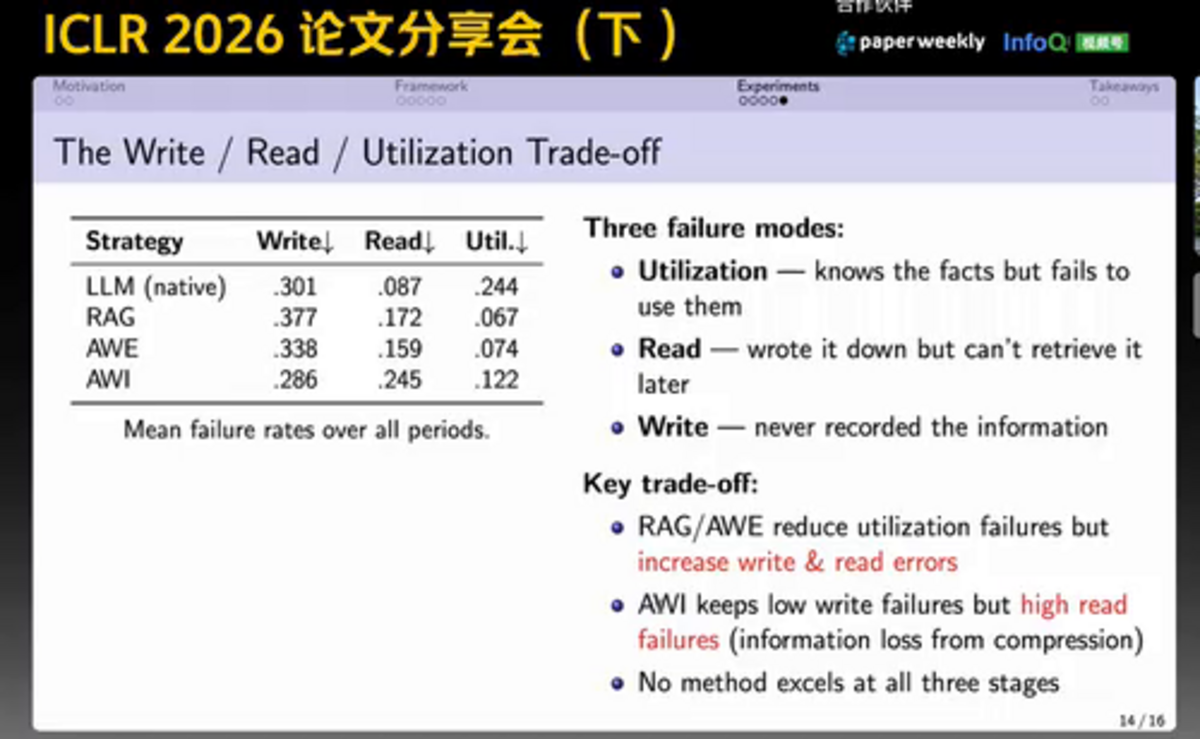
\includegraphics[width=0.82\linewidth,height=0.34\textheight,keepaspectratio]{figures/fig09_failure_tradeoff.png}
  \caption[write、read、utilization 三类 failure 的 trade-off]{write、read、utilization 三类 failure 之间存在 trade-off，RAG/AWE 降低 utilization failure，同时增加 write 和 read 错误。\protect\footnotemark}
  \label{fig:failure-tradeoff}
\end{figure}
\footnotetext{视频时间：00:17:50--00:18:59。}

视频明确给出的总体变化是：RAG 和 AWE 将 utilization failure 从约 24\% 降到约 7\%。这个结果说明外部记忆能帮助模型把已有事实用到答案里。代价也清楚：write 和 read 错误会上升。AWI 的写入失败率保持较低，可是 read failure 很高，视频解释为压缩进自身上下文时丢失了很多重要信息。

视频随后给出诊断层面的优化线索：memory-write/update frequency 越低，read failure 往往越高，可能原因是本地 retained local messages 过多，读取时容易混淆该用哪条事实。speaker 还点到 noise 与 top-k 两个旋钮：检索噪声会把无关片段带回 context，top-k 过小可能漏掉关键事实，top-k 过大又会增加干扰。视频没有展开完整消融，所以这里把它们作为调参方向记录，核心含义是诊断指标能把优化从“总分低”推进到“该调写入频率、检索干净度还是返回条数”。

\begin{warningbox}{三环节权衡}
外部记忆设计没有免费午餐。把所有内容都存起来，会增加检索噪声；让 agent 自主筛选，会依赖写入策略的质量；把内容压缩进 context buffer，会承担细节丢失风险。AMemGym 的价值在于把这些失败拆开，让优化目标从“总分变高”转向“到底是哪一环坏了”。
\end{warningbox}

\subsection{本章小结}

本章的实验发现是，external memory 的收益真实存在，RAG/AWE 能把 utilization failure 从约 24\% 降到约 7\%；与此同时，write/read/utilization 三环节之间会发生失败转移。AWE 在视频对比中最均衡，RAG 的检索结果可能 noisy，AWI 的压缩路径存在信息丢失问题。诊断层面还要观察 memory-write/update frequency、retained local messages、noise 与 top-k，因为这些旋钮会改变 read failure。ASR 中的 “RNG” 按上下文校正为 `RAG`，`AWI` 和 `AWE` 均按视频中的 external memory 机制解释，未补写视频没有明确给出的模型名单、公式或额外数值。
